\documentclass{article}

\usepackage[utf8]{inputenc}
\usepackage{amsmath,amssymb}
\usepackage{graphicx}
\usepackage{booktabs}
\usepackage{hyperref}
\usepackage[margin=1in]{geometry}

\title{FarmBot Automated Imaging Extension}
\author{Bryan Portillo}
\date{\today}

\begin{document}

\maketitle

\begin{abstract}
This document describes an extension to FarmBot OS for configurable,
periodic image collection across registered plants.
\end{abstract}

\section{Introduction}

The extension adds an operating-system-level imaging service rather than
requiring users to reprogram an experiment for each collection run.

\section{Architecture}

The system consists of a supervised photo collection service, a plant data
provider, a hardware movement adapter, a camera registry, and a frontend
configuration panel.

\section{Scheduling}

The next execution time is modeled as

\begin{equation}
T_{\text{next}} = T_{\text{completed}} + \Delta t.
\end{equation}

\begin{figure}[t]
    \centering
    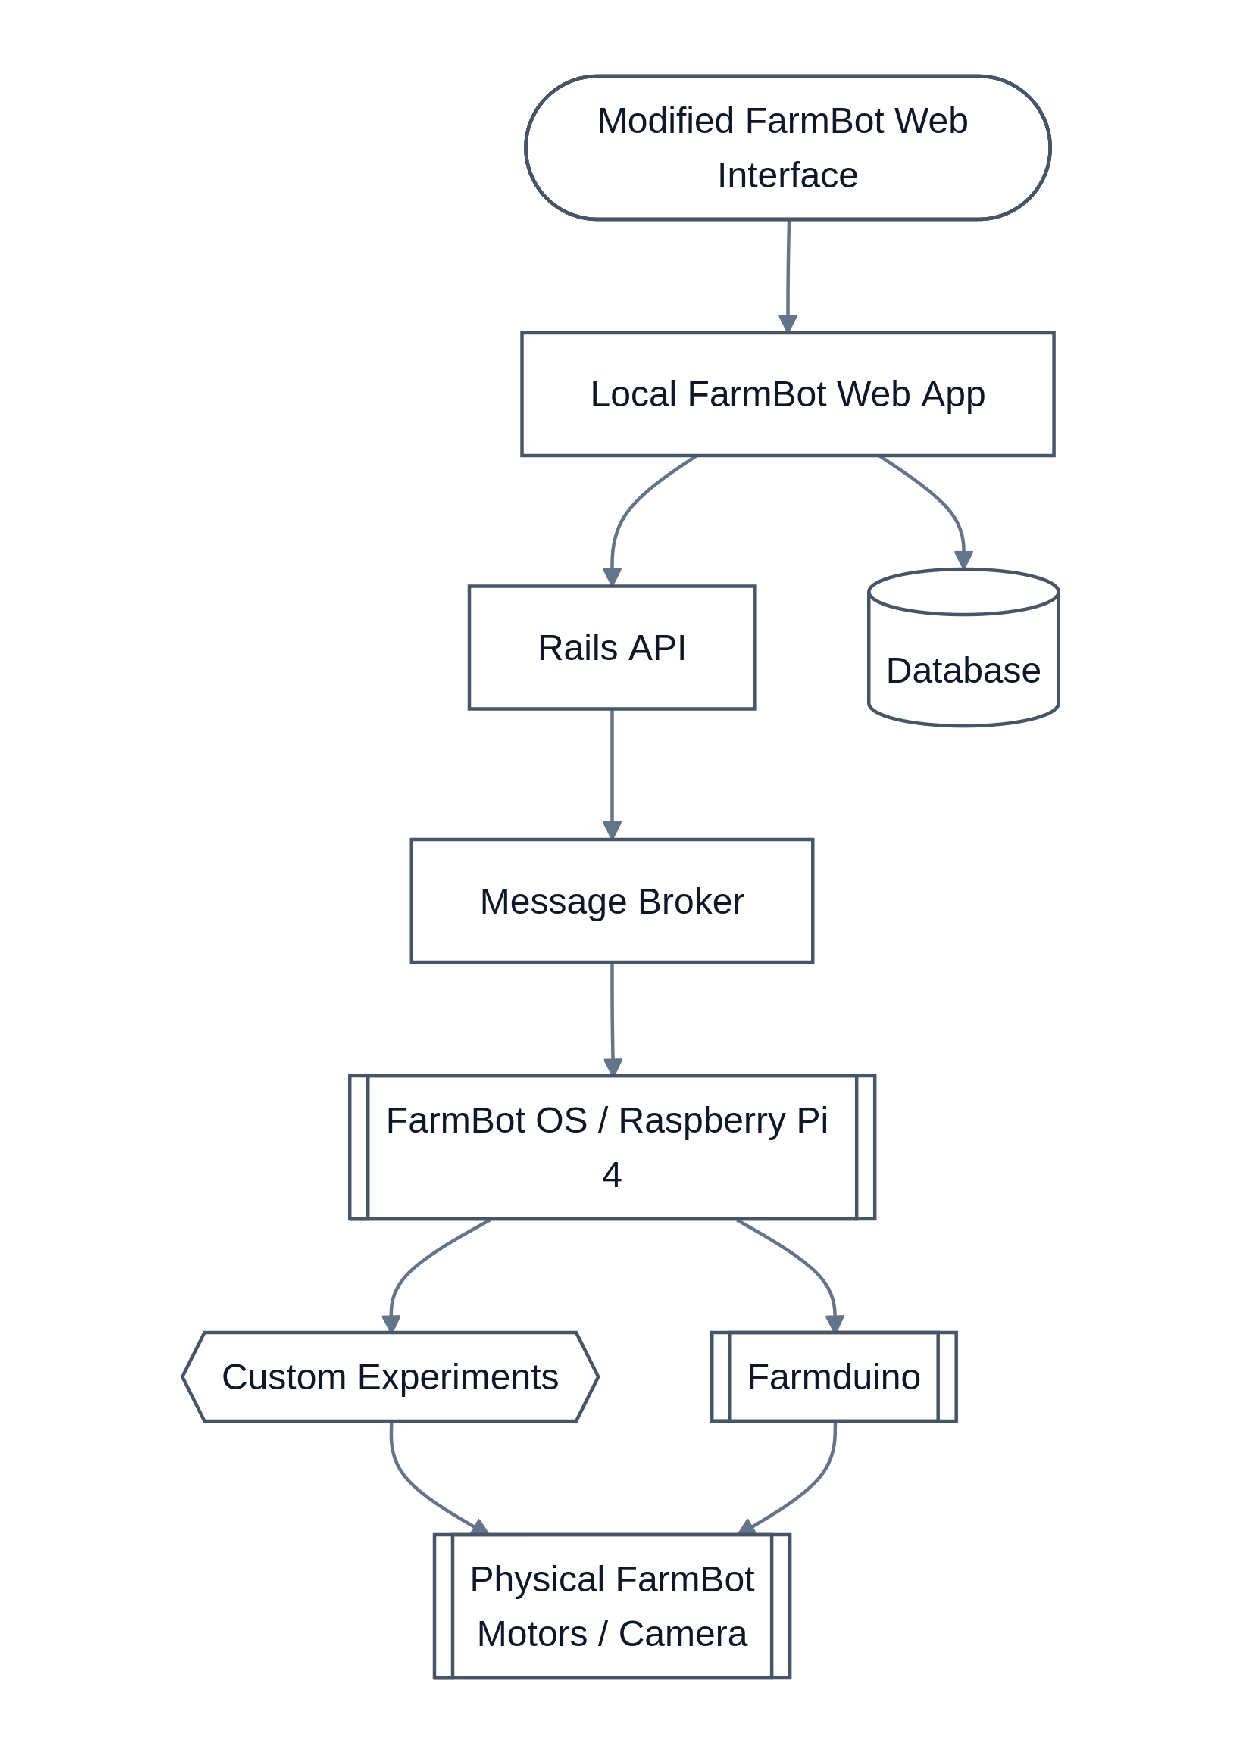
\includegraphics[width=\linewidth]{figures/architecture.pdf}
    \caption{FarmBot architecture.}
    \label{fig:farmbot-architecture}
\end{figure}

\begin{figure*}[t]
    \centering
    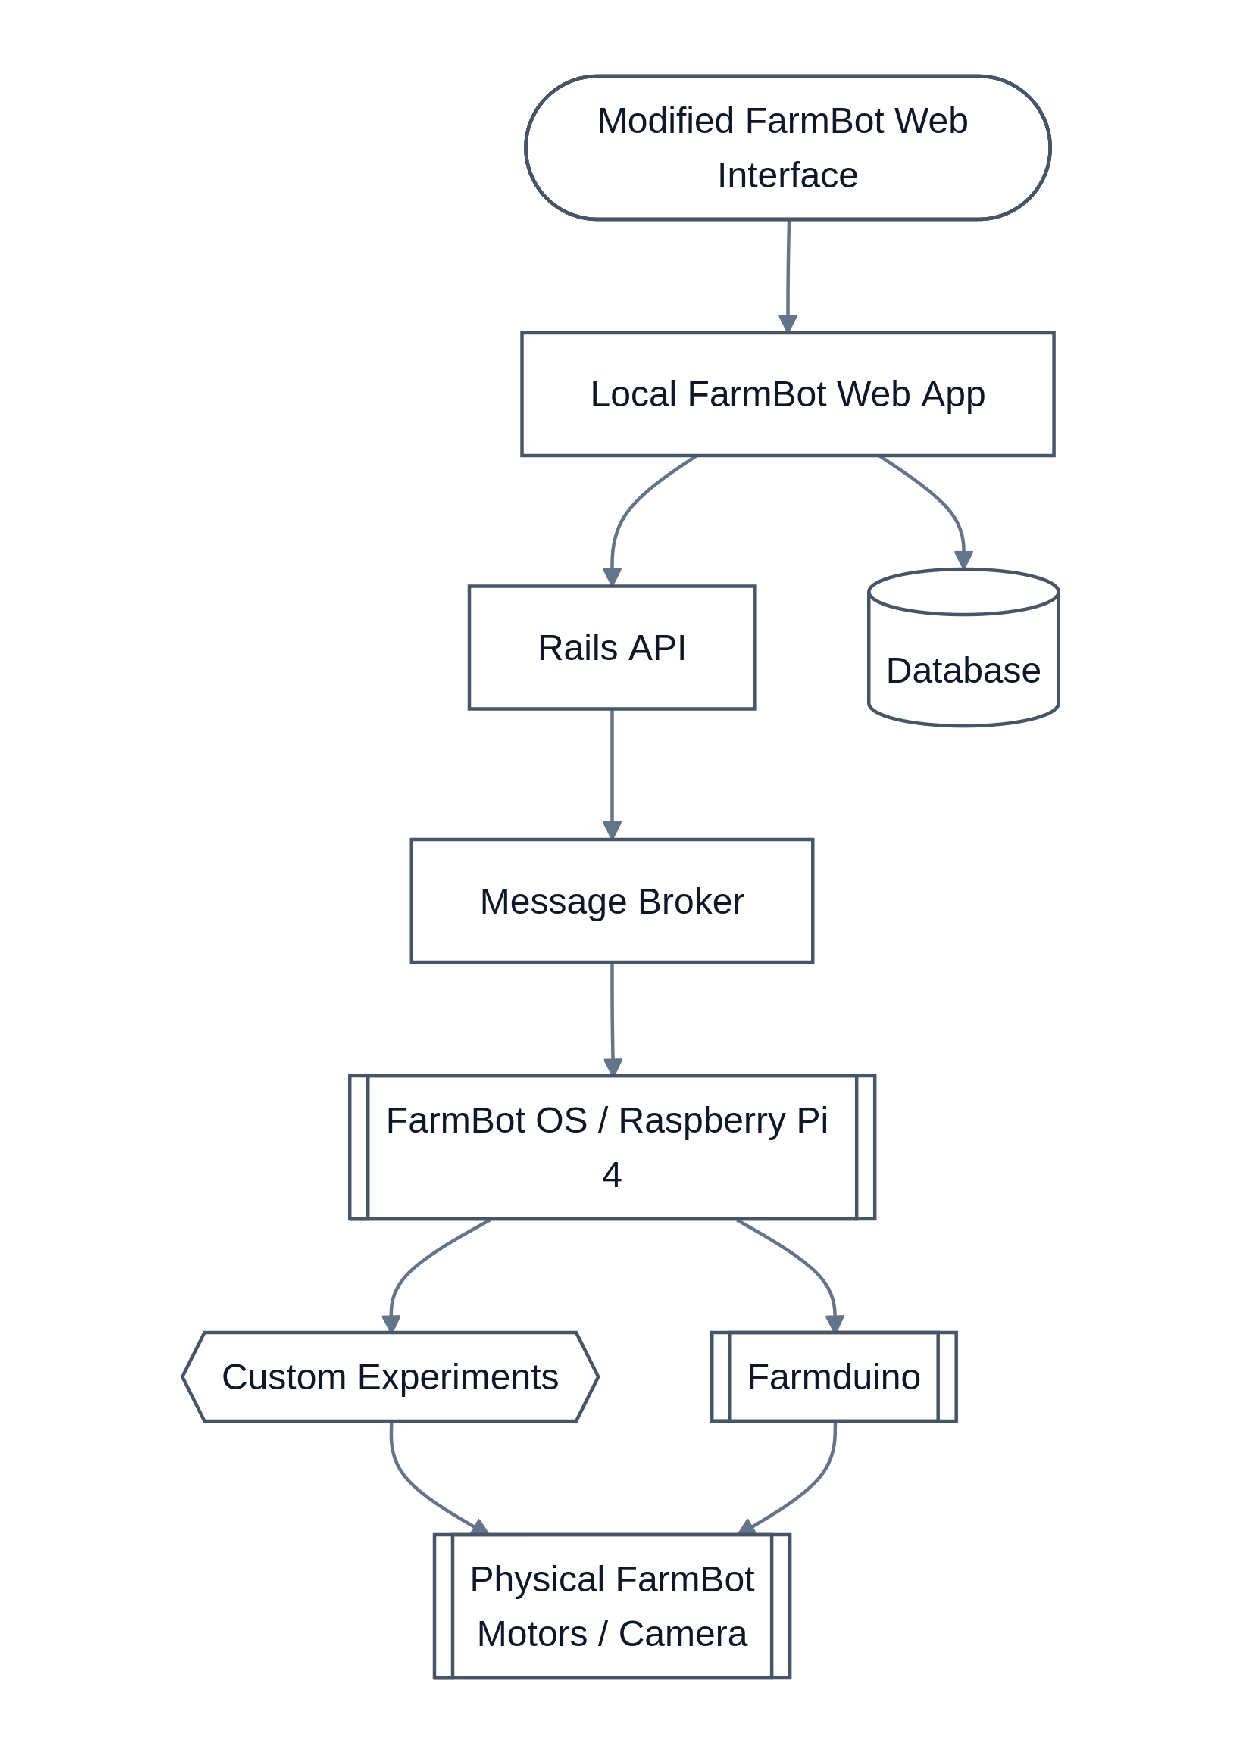
\includegraphics[width=\textwidth]{figures/architecture.pdf}
    \caption{FarmBot architecture.}
    \label{fig:farmbot-architecture}
\end{figure*}

\section{Implementation Status}

The backend command surface, Lua integration, local web server, and frontend
controls have been implemented. Physical validation is the remaining
deployment milestone.

\section{Conclusion}

The design establishes automated imaging as a reusable FarmBot capability
that can later support additional cameras and sensing workflows.

\bibliographystyle{plain}
\bibliography{references}

\end{document}
